\chapter{Design and Prototyping}\label{ch:DesProt}\addtocontents{lof}{\protect\contentsline{chapter}{\protect\numberline{\thechapter}Methodology}{}{}}
\vspace{-2.5em}
% \newthought{Synopsis}\synopsisChProcessing
\marginpar{
    \centering
    \footnotesize
    \includegraphics[width=\linewidth]{figures/flat.png}
    \captionof{figure}{Flat Valve Model}
    \label{fig:flat}
}
\marginpar{
    \centering
    \footnotesize
    \includegraphics[width=\linewidth]{figures/balloon.png}
    \captionof{figure}{Billowed Valve Model}
    \label{fig:ballon}
}
\marginpar{
    \centering
    \footnotesize
    \includegraphics[width=\linewidth]{figures/balloont.png}
    \captionof{figure}{Billowed Valve with Chordae Tendineae Model}
    \label{fig:ballont}
}
\marginpar{
    \centering
    \footnotesize
    \includegraphics[width=\linewidth]{figures/anat.png}
    \captionof{figure}{Anatomical Model}
    \label{fig:anat}
}
\newthought{Synopsis}\synopsisDesign
\mynewline
\section{Conceptualisation and Initial Design}
The essence of a design process is inherently iterative and exploratory. It takes form of a cycle of conception, experimentation, evaluation, and refinement. This iterative cycle is fundamental to translating abstract ideas into tangible solutions that meet set goals.
%Within this framework, the development of a mock \gls{TV} for a heart simulator exemplifies the complex interplay of innovation, precision, and adaptability.

At the heart of the design process lies trial and error—a methodical yet flexible approach that takes discovery of unexpected challenges and leverages them as opportunities for learning and input. Initial ideas are transformed into preliminary models, serving as the first step in a series of continuous interactions between designing, testing, and iterating.
%This process is characterized by the application of various modeling approaches, each iteration informed by the insights gained from previous attempts and the evolving understanding of the project's objectives.

The dynamic nature of this process sets a strong base to pivot strategies, incorporate new technologies/materials, and adapt to findings in real-time. The design changes throughout this project were not merely reactions to setbacks but were driven by a pursuit of optimization whether in response to material limitations, fabrication challenges, or new modelling insights.
% Reworking based on these design changes is critical, allowing the prototypes to improve incrementally, each iteration bringing them closer to the optimal balance between theoretical accuracy and practical functionality.


\mynewline
The initial vision of the in-vitro \gls{TV} was formed on reflection of the literature review. It is crucial to consider both the anatomical fidelity required for effective simulation and the technical feasibility of creating a functional model when developing initial concepts which can then be adapted as the project moves forward and firmer boundaries are discovered.

The approach taken was to start prototyping with the simplest design and gradually increase complexity as the project progressed. This allowed for a more systematic exploration of the design, ensuring that each iteration built upon the insights gained from the previous one with respects to all stages of manufacturing and a minimal time investment in preliminary modelling so the prototyping process could be refined in tandem. This was essential to finishing with a refined final model, balancing anatomical fidelity with fabrication feasibility and functional performance.

\section{Design Criteria}\label{sec:Design Criteria}
The design criteria were established to guide the development of the mock \gls{TV}. These criteria were informed by the project's objectives, the gaps in the literature, and the technical constraints of the fabrication process.
% \mynewline
The design criteria were as follows:
\begin{fullwidth}
    \newthought{Criterion 1: Anatomical Fidelity}\\ The mock \gls{TV} should precisely resemble the anatomical structure of the \gls{TV}, capturing the key features of the valve's leaflets, annulus, and chordae tendineae and where possible to account for the variations.
    \begin{itemize}
        \item Justification: To maintain a realistic simulator effort must be made to ensure represenative geometry to provide a realistic evaluation tool for medical devices.
    \end{itemize}

    \newthought{Criterion 2: Functional Performance}\label{sec:Functional Performance}\\ The mock \gls{TV} should exhibit the functional characteristics of the \gls{TV}, including the ability to open and close in response to fluid flow, and the capacity to simulate regurgitation simulating the physiological and pathological conditions of a natural \gls{TV}.
    \begin{itemize}
        \item Justification: Without these functional characteristics, the mock valve would be limited in applicability for integration and characterisation of a prosthetic valve device.
    \end{itemize}

    \newthought{Criterion 3: Material Compatibility}\\ The materials used in the fabrication of the mock \gls{TV} should be flexible, durable, and suitable for the intended application, ensuring that the valve can withstand the fluid flow and mechanical stresses.
    \begin{itemize}
        \item Justification: The valve, once integrated into the right heart simulator, will be subjected to continuous fluid flow and mechanical forces over a long period of time, necessitating the use of materials that can withstand these conditions over a long period of time.
    \end{itemize}

    \newthought{Criterion 4: Fabrication Feasibility}\\ The design of the mock \gls{TV} should be amenable to the fabrication process, considering the limitations of the 3D printing and moulding techniques used in the project.
    \begin{itemize}
        \item Justification: Some aspects of \gls{TV} performance are depenedent on biological factors that are difficult to replicate such as collagen fiber allignment. This design should be able to be fabricated in a way that can be easily replicated and improved upon in the future.
    \end{itemize}
    %While also being a key point to the larger project of the heart simulator the valve should be easily replicated and improved on upon again in the future.
    \newthought{Criterion 5: Scalability and Modifiability}\label{sec:Scalability}\\ The design of the mock \gls{TV} should be scalable, allowing for the creation of multiple valve moulds easily by hot-swapping the scanned and refined \gls{CT} models with varying anatomical features and functional characteristics
    \begin{itemize}
        \item Justification: As the overarching project of the right heart simulator progesses past this thesis the valve should be easily replicated and improved upon again so that future goals can be met.
    \end{itemize}
\end{fullwidth}

\section{Modelling and Design Iterations}

\subsection{Simplified Valve Designs}

\newthought{Flat Valve:}
As illustrated in \cref{fig:flat} the flat valve was the first to be developed with the idea being to use it as a basis for developing the complexity. The shape of the leaflets were designed by overlaying images of regurgitant valves from a study which modelled the \gls{TV} at different stage of regurgitation \citeonly{namModelingTricuspidValve2023} in systole normal to the annulus of the valve over a disc in SolidWorks and then drawing a spline aligned with the leaflet shapes.
In later iterations of this basic structure considerations started to be made for the chordae tendineae, whether to include them or not and then how. There was two schools of thought for this method:
\begin{itemize}
    \item Having the tendineae attached within the mould and casting the part all of the same material.
    \item Casting the valve part without tendineae and then attaching tendineae after made from another material.
\end{itemize}
It wasnt until outcomes in the prototyping phase, section:\cref{sec:Chord}, that the this was fully decided on based off of experimental results.
%as studies from the literature review \todo{reference} showed how the elastic modulus varied greatly from leaflet to  tendineae.

\newthought{Billowed Valve:}\\
The next layer of complexity for the valve to visually replicated an anatomical valve was adding the billowed effect.
The literature review section:\cref{sec:varpath} showed how in reguritant valves the annulus dilates, tendineae weaken and valve develops a partial prolapse, this was reflected in later iterations by creating a revolve feature in SolidWorks in a 'U' shape which was centered within the leaflets (as opposed to the annulus) to overlay the cusp cut on top of.
\begin{figure}
    \centering
    \includegraphics[width=0.8\textwidth]{figures/billow}
    \caption{Visual represenation of regurtitant valve morphological progression \citeonly{namModelingTricuspidValve2023}}
    \label{fig:bill}
\end{figure}
% It was hoped with the added depth to the leaflets in this iteration that the valve would be able to coapt as the cusps began to have more overlap with adjacent leaflets
Later iterations of this model included the chordae tendineae, and added extrusions on the leaflet cusps to allow the leaflets to coapt properly however as prototyping progressed and the possibility for using a model converted from a \gls{CT} scan grew brighter, the work on the representative models was put on hold.


\subsection{Represenative Valve Designs}

\newthought{Anatomical Valve Model:}\\
While development on the mock valve was progressing the idea for a more anatomically accurate valve began to look favourable for it aligned more closely to the aims of the project. The idea was to use a \gls{CT} scan of a \gls{TV} and then convert this into a 3D model. There was a few options on how to do this, a software package like Mimics can be used to do it easily however this package is very expensive or open source programs like Ostrix. Due to the dificulties in capturing the geometry of tricuspid valves in \gls{CT} and the less user friendly interface of Osirix it was decided that a pre-existing model from an online STL repository would be used as a base instead and then refined to fit the project's needs.

With this approach the tracability of the model is lost but with confirmation from the designer that is was developed off of imaging from a human it was deemed fit for purpose.

\mynewline
Harnessing the converted model presented many unexpected challenges, this was discovered when initially trying to import the STL model into SolidWorks a large amount of zero thickness geometries were present. The main technical issues with this model were:
\begin{itemize}
    \item Self-intersecting faces,
    \item Non-manifold edges
    \item Holes throughout the surface
    \item Inaccuracies in the model
    \item Widely varying leaflet thickness
\end{itemize}
The development of this model had been originally intended to provide educational illustrations of the anatomy not to be produced physcially so work began to refine it for physical production.

\subsection{Model Refinement}
In tackling these issues and getting the converted model to a usable state there was a number of softwares tried and tested to see which could effectively resolve the issues. The main softwares used were Meshlab, Meshmixer, Blender and AutoCAD NetFabb and SolidWorks.

Meshlab is an open-source software that is used for processing and editing unstructured 3D triangular meshes. Mesh-lab is a very low-level\sidenote{Low-level programming involves direct manipulation of hardware resources, offering granular control but requiring detailed hardware knowledge.} program,  it was used to try and remove the non-manifold edges however the methods to do so require knowledge of advanced mathematical equations and how to manipulate them. With initial attempts and references to online tutorials resulting in the model being distorted and unusable, the decision was made to find a more user-friendly software.

% With concerted effort MeshLab might have been able to resolve the issues but with many options on the market it was thought that looking elsewhere would be more beneficial. 

AutoCAD NetFabb seemed a fitting replacment as mentioned in many only forums discussing MeshLab's limitations. Originally designed for additive manufacture pre-processing it also contained a diverse suite of usefuls tools to repair the model. Personalized repair kits could be designed to fix specific issues for the \gls{TV} and most importantly had been developed for higher-level applications.
\begin{itemize}
    \item Repair Scripts
          \begin{figure}[H]
              \centering
              \includegraphics[width=0.8\textwidth]{figures/NetFabbRepair.png}
              \caption{Netfabb Repair Scripts}
              \label{fig:NetfabbRepair}
          \end{figure}
    \item Shell
          \begin{figure}[H]
              \centering
              \includegraphics[width=0.8\textwidth]{figures/NetFabbShell.png}
              \caption{Netfabb Shell Tool}
              \label{fig:NetfabbShell}
          \end{figure}
\end{itemize}


After the repairing and hollow shell process was complete the model was in a state to trial some prototyping methods, the model was given a retainer ring to allow for easy mounting and printed with a FormLabs \gls{SLA} printer. From initial attempts at fabrication using the silicone moulding method it was evident that casting the tendineae would not be feasible so a tool within NetFabb was found to remove them from the geometry.w
\begin{figure}
    \centering
    \includegraphics[width=0.8\textwidth]{figures/nfcut}
    \caption{Netfabb Cutting Tool}
    \label{fig:Netfabbcut}
\end{figure}

From here the model was imported into Blender to further refine the model as NetFabb was not capable of detailed mesh sculpting to refine the model by hand. In blender the main objective was to smooth out the bumps in the leaflets left from the cuts and to ensure the leaflets were of a uniform thickness without straying off the original geometry too much. 

Meshmixer was used in tandem with blender as it contained a very useful thickness analysis tool which could be used to see the varying thicknesses of the leaflets in the imported model, Blender was then used to manually edit the model using its sculpting tools to either thicken or thin the surface where appropriate. This would have been much easier if a dynamic thickness overlay had been developed in Blender and attempts to do so were made but as the coding for personalized tools in the open source program wasn't well documented it was abandoned for the former method.





Once the final valve model was finalised the decision was made to flatten the saddle-shape of the geometry to simplify the moulding and mounting processes, some surgical studies like \citeonly{mahmoodChangesMitralValve2010} showed that for mitral valves it does have a structural disadvantage however this did not reduce the ability to coapt properly.



% Physical prototyping:

% Printing errors
% Moulding errors
% Material errors
% Assembly errors
% Design errors

% Tools:

% 3D printer
% Spatula
% Syringe
% Precision blade
% Sanding paper
% Pliers
% Tweezers

\section{Prototyping}
\subsection{Valve Iterations}
\newthought{Preliminary Prototyping Methods}
The prototyping method went through a few key stages, throughout the simplified valve modelling stage the running methods were creating \gls{PLA} prints of the flat and billowed valve models and then using a silicone mould to capture its likeness, through feasability testing it was found this method was not suitable for as;
\begin{figure}
    \centering
    \includegraphics[width=0.45\textwidth]{figures/silicone mould}
    \includegraphics[width=0.45\textwidth]{figures/silicone mould open}
    \caption{Silicone Mould Design}
    \label{fig:silimould}
\end{figure}
\begin{itemize}
    \item Silicone moulds could not hold firm enough in casting to maintain sub 1mm thicknesses.
    \item The mould release agent was less effective on \gls{PU}-Silicone interfaces than expected.
    \item The moulds even with appropriate vent holes and degassing would still have large air bubbles and not fill out to the edges of the part.
\end{itemize}
As it seemed no amount of optimization of this method would improve results further work was done to find a more suitable method.

\newthought{Press Moulding}
This new method involved designing blocks in SolidWorks as a separate body to the valve part and using the 'Combine' tool to subtract the valve part. This hollowed block could then be split in the middle to create a two-part mould.\\
The \gls{PU} resin could then be poured into the cavity part and the lid part pressed ontop with a C-clamp to create a tight seal.
\mynewline
This method was trialed on the simplest flat valve model to seek learnings for my complicated designs, some such learning were;
\begin{itemize}
    \item To measure the volume of the 2-part casting fluid with a precision scales as opposed to doing by eye, having the mixture slightly off resulted in gross discolouring and an extremely sticky surface.
    \item To come up with a new chordal attachment method as the trialed insertion buds were inneffective.
\end{itemize}
\begin{figure}
    \centering
    \includegraphics[width=0.45\textwidth]{figures/flat mould}
    \includegraphics[width=0.45\textwidth]{figures/flat valve}
    \caption{Press Mould Design and casted part for Flat Valve}
    \label{fig:flat mould}
\end{figure}

\mynewline
As the modelling stages evolved in complexity so did the prototyping, in trialing preliminary anatomical valves for press moulds it was discovered that due to STL interaction issues with solid \gls{CAD} geometries the valve could not be moulded directly and so a mould die was designed and prototyped of the valve part mould die, making it a two step process to work around this modelling issue.

A deep-cast epoxy was used to pour into these die so form the moulds for the valve, key learnings from this process were;
\begin{itemize}
    \item Thin, easily breakable walls for the mould die were imperative as the epoxy parts were dificult to remove, this had a downside of making the die single use. This was hoped to be avoided with notches to pry the epoxy part out but ultimately wasn't effective.
    \item A split mould was trialed as it was thought to make demoulding the casted part easier however this resulted in significant lines being apparent and didn't help significantly in demoulding so it was abandoned.
    \item Embossing and debossing key slots in the die ensured the moulds could be aligned correctly with ease.
    \item Sanding down the \gls{PLA} prints to a smooth finish so in combination with a mould release grease greatly eased the demoulding of the die.
    \item Initial drafts of mould die joined the cusps of leaflets directly however it was found that extruding the cusps axially stopped excess material from curing past the cusp of the leaflet and also acted as a central large key slot for pressing the moulds into eachother.
\end{itemize}
% \begin{figure}
%     \centering
%     \includegraphics[width=0.45\textwidth]{figures/firstdraftmouldofmould}
%     \includegraphics[width=0.45\textwidth]{figures/firstdraftcastedpart}
%     \caption{Press Mould Design and casted part for Flat Valve}
%     \label{fig:flat mould}
% \end{figure}
\begin{figure}
    \begin{fullwidth}
        \centering
        \subfloat[First draft mould die]{%
            {\includegraphics[width=0.45\linewidth]{figures/firstdraftmouldofmould}}%
        }\quad
        \subfloat[Later iteration of mould die]{%
            {\includegraphics[width=0.45\linewidth]{figures/mouldofmould}}
        }
        \quad
        \subfloat[Split mould trialing]{%
            {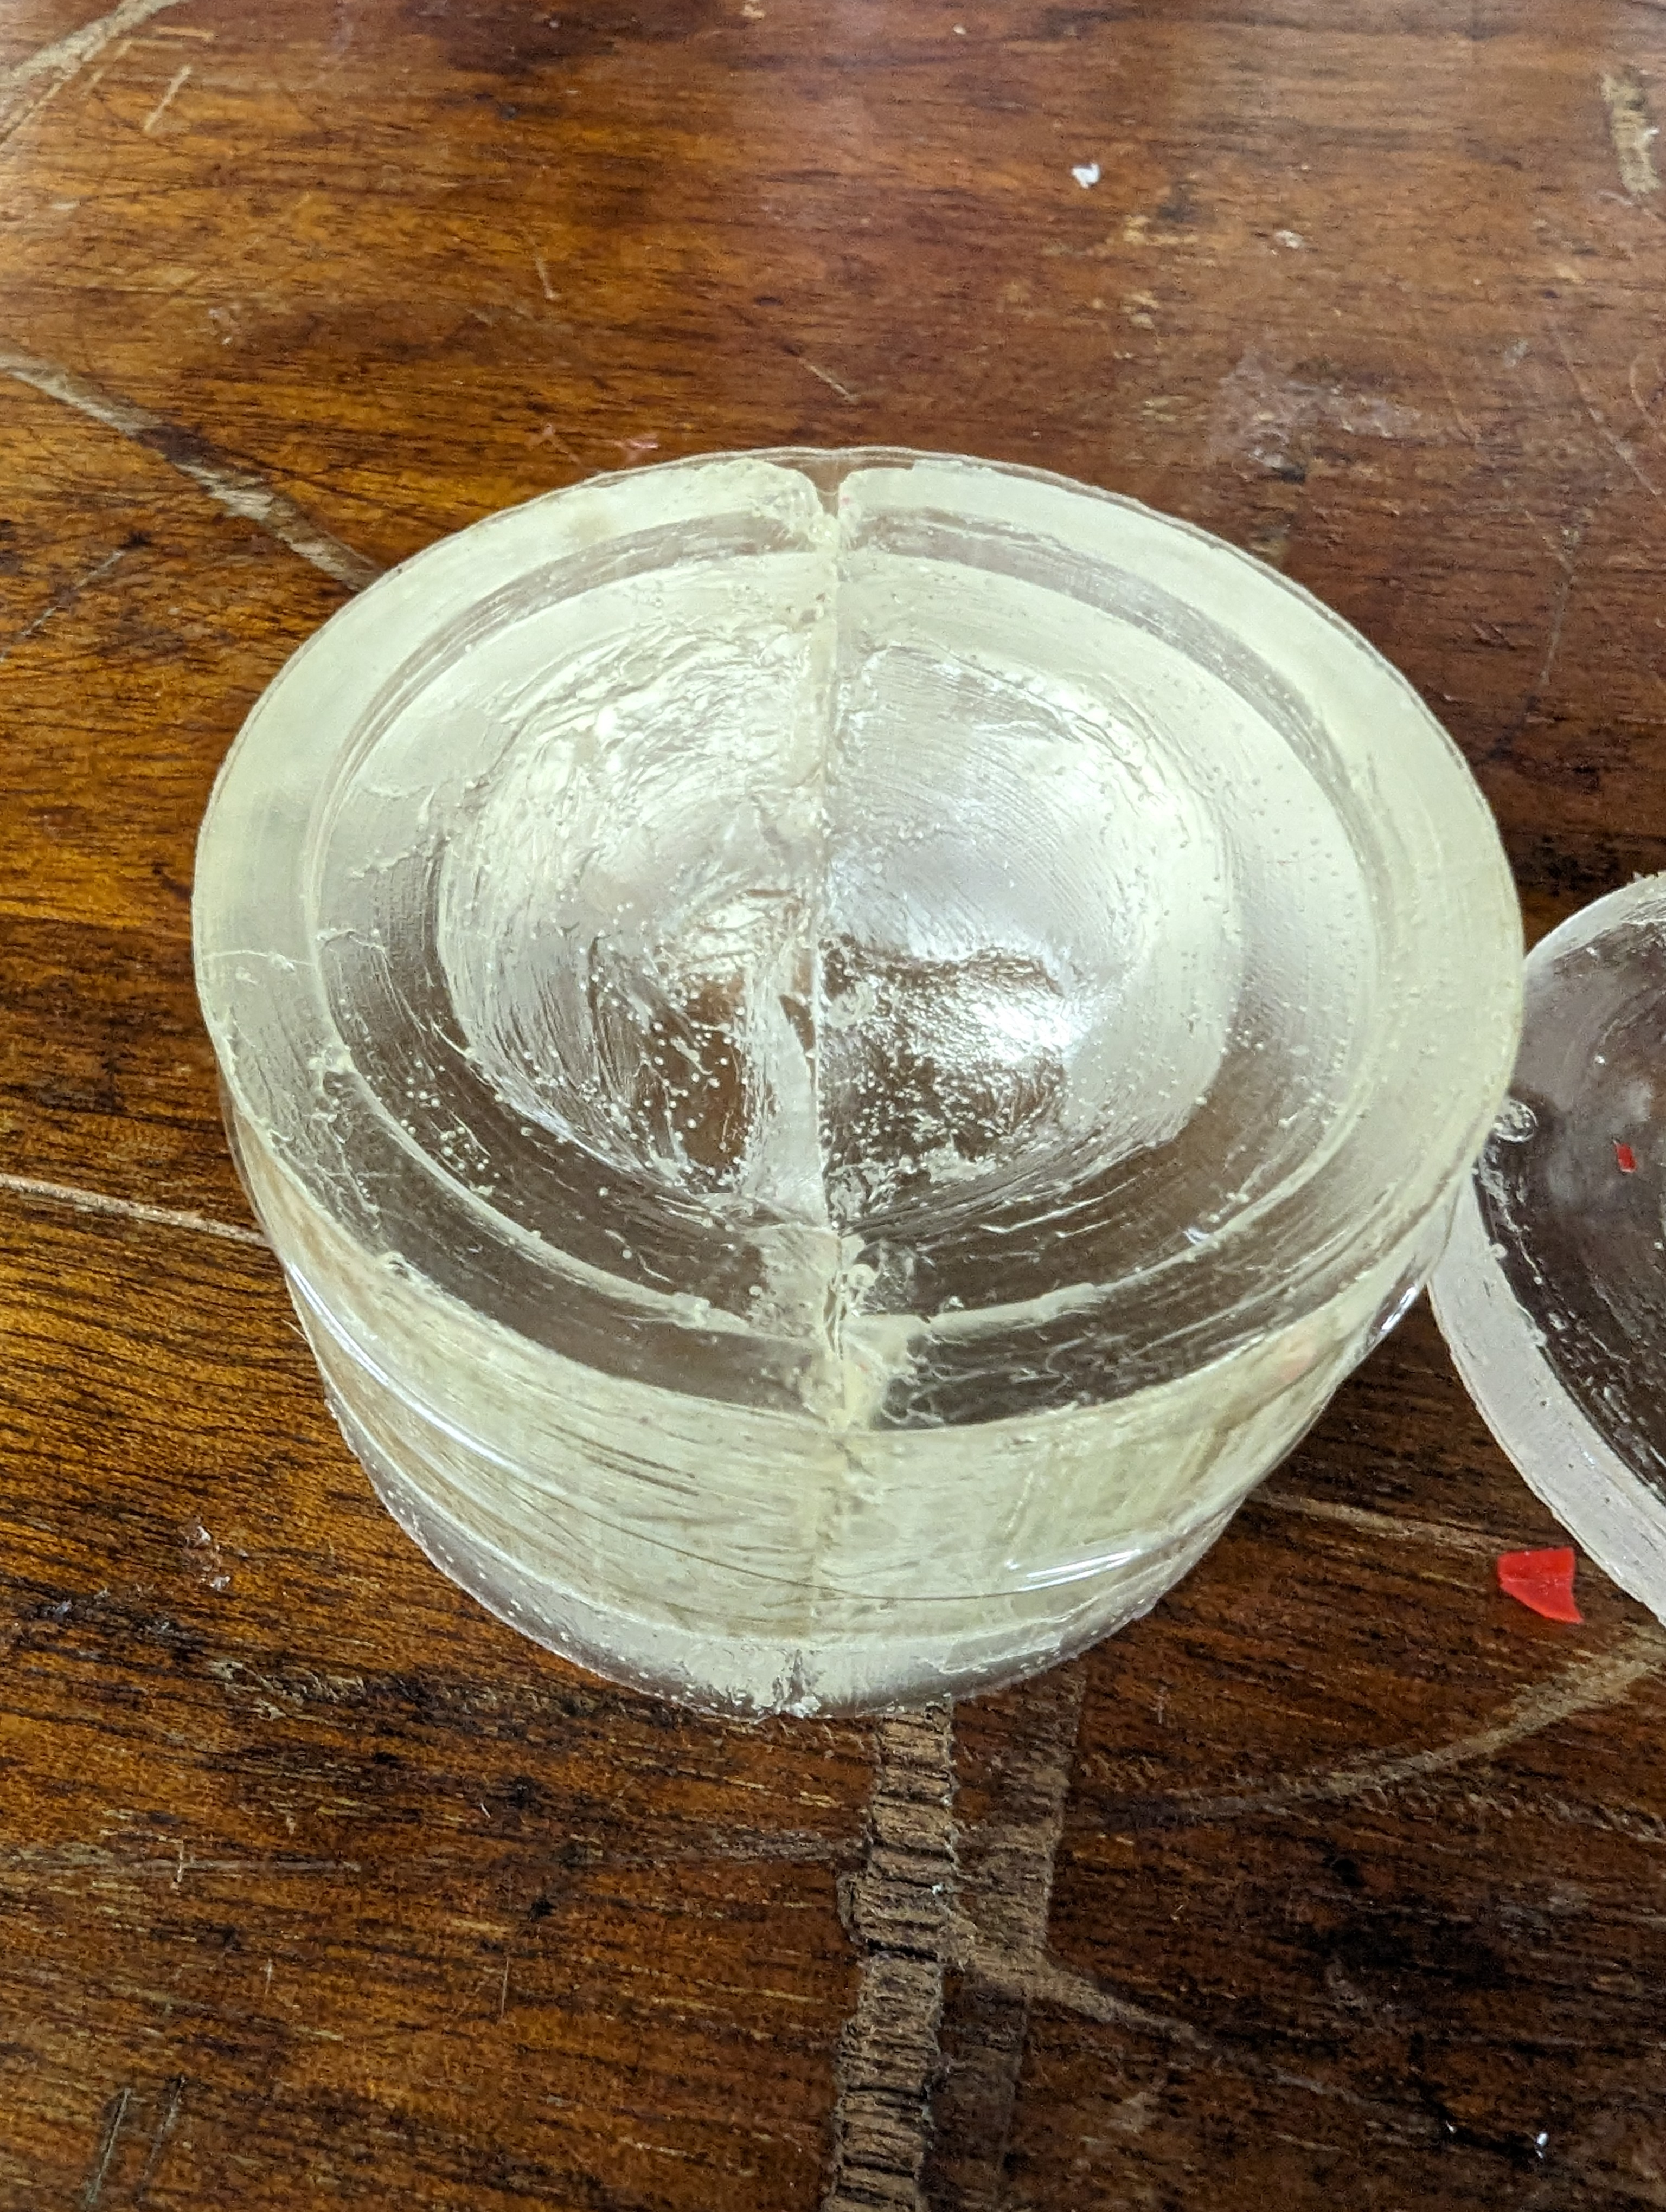
\includegraphics[width=0.45\linewidth]{figures/splitmoulddesign}}
        }
        \quad
        \subfloat[Draft and casted part of epoxy moulds]{%
            {\includegraphics[width=0.45\linewidth]{figures/firstdraftcastedpart}}
        }
        \caption{Iterations of epoxy mould die method}
        \label{fig:moulddie}
    \end{fullwidth}
\end{figure}

% Materials used:

% Platinum cure silicone
% Polyurethane resin
% Ecolex transparent silicone
% Epoxy
% PLA
% SLA resin
% B7000 adhesive
% Nylon write
% Mould release
% Grease
% Isopropyl alcohol
\subsection{Chordae Tendineae}\label{sec:Chord}
Initial conceptualization of the chordae tendineae involved having the valve as one homogenous material with the tendineae attached within the mould. However, as the project progressed and the complexity of the valve increased, it was decided that the tendineae should be a separate part that could be attached after the valve was cast. This was decided on as the elastic modulus of the tendineae was vastly different as they function to be pulled taught to stop the leaflets from prolapsing.

\newthought{Design of Choice:}
A 0.1mm nylon fishing wire was chosen to represent the tendineae as it was thin enough to be completely collapsible and not interfere with the opening in the diastolic phase.
The attachment to the valve was the more challenging aspect, a few methods were considered and tested:
\begin{figure}[H]
    % \begin{fullwidth}
    \centering
    \subfloat[Embedded method trialing]{%
        {\includegraphics[width=0.45\linewidth]{figures/embeds}}%
    }\quad
    \subfloat[Cyanoacrylate method trialing]{%
        {\includegraphics[width=0.45\linewidth]{figures/embedswithgluesamp}}
    }
    %   \quad
    %   \subfloat[Split mould trialing]{%
    %     {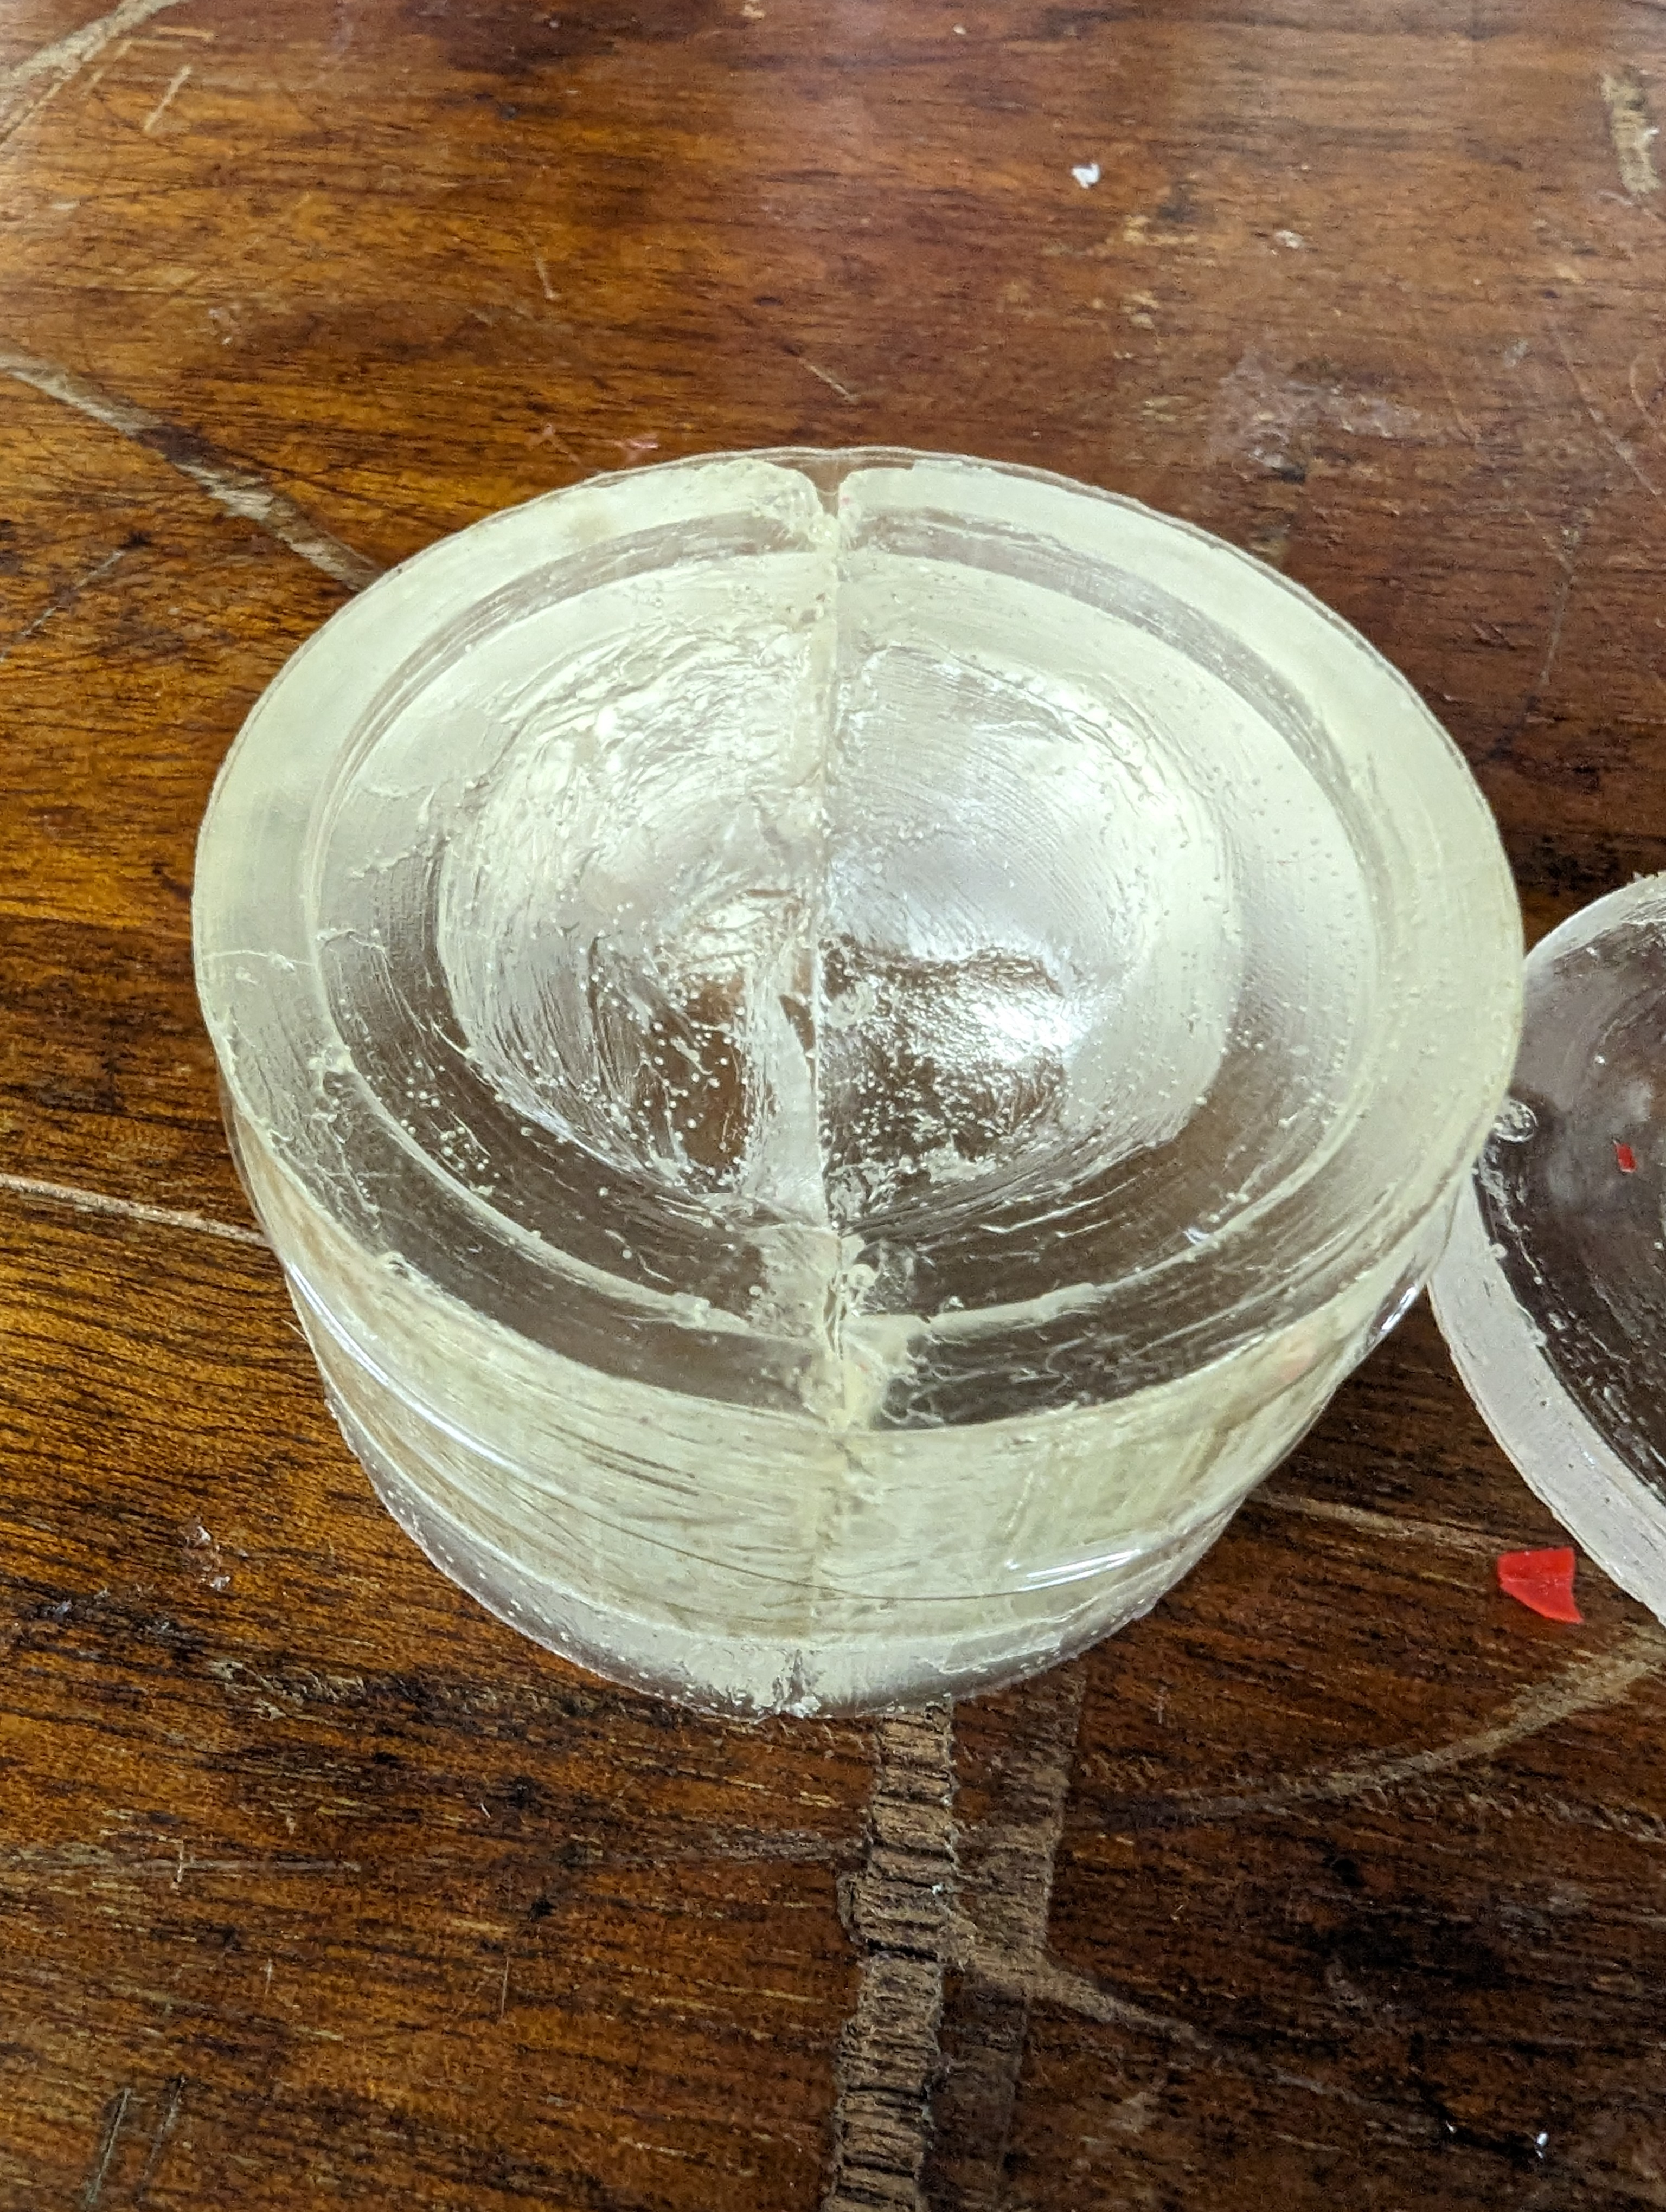
\includegraphics[width=0.45\linewidth]{figures/splitmoulddesign}}
    %   }
    %   \quad
    %   \subfloat[Draft and casted part of epoxy moulds]{%
    %     {\includegraphics[width=0.45\linewidth]{figures/firstdraftcastedpart}}
    %   }
    \caption{Testing the methods for attaching the chordae tendineae to leaflets}
    \label{fig:ctattachment}
    % \end{fullwidth}
\end{figure}
\begin{itemize}
    \item Suture patterns along the cusp of the leaflets.
          \begin{itemize}
              \item A short continuous suture was used to attach a few tendineae to the leaflets on a sample piece of \gls{PU} how on a gentle tensile test the suture ripped out as the \gls{PU} wasn't strong enough to hold.
          \end{itemize}
    \item Using a small hole in the leaflet to thread the tendineae through and then knotting it on the other side.
          \begin{itemize}
              \item This method also failed as the elasticity of the \gls{PU} made it so the knot would have to be \gls{PU} would rip anyway.
          \end{itemize}
    \item Embedding the wire in the \gls{PU} leaflets.
          \begin{itemize}
              \item While hopeful the embedding technique proved not feasible as the wire just slipped out, there was an attempt made with thick and thin layers of additional \gls{PU} but to no avail.
          \end{itemize}
    \item Gluing the tendineae to the leaflets with a cyanoacrylate adhesive.
          \begin{itemize}
              \item While this method showed initial promise as the adhesive was strong enough to hold the tendineae after seconds of curing, when 24 hours passed the adhesive would harden much stiffer and deform the leaflets making them very rigid.
          \end{itemize}
    \item Gluing with B7000 adhesive.
          \begin{itemize}
              \item The B7000 adhesive was chosen as it was a flexible adhesive, initial tests werent fruitful but if left to set fully over 24 hours the bond became very strong and the leaflets retained their flexibility while also only needing a miniscule amount for a good hold so the very thin thickness of the leaflets wasnt negated.
          \end{itemize}
\end{itemize}

\subsection{Fixturing}
The design criterion was considered carefully before modelling the test fixturing. The main desired outcomes from the testing that the fixturing should facilitate were:
\begin{itemize}
    \item The chordae tendineae should have anchors which are fully adjustable axially and angularly to allow for a range of testing positions.
    \item The valve should be mounted in a way that the leaflets are not obstructed so the valve can be viewed from multiple angles for thorough evaluation.

\end{itemize}

\newthought{Design of Choice:}
A combination of 3D printed parts, off-the-shelf components and hand-cut threaded rods were used to emulate the initial sketch of the rig

The threaded rods allowed for the anchoring points of the tendineae to be adjusted axially.

Attached to the rods was the ring system with notches that could be adjusted angularly which the mock tendineae were passed through and fastened to with a rubber wedge.


\section{Design Validation}
To investigate the experimental thickness of the valve model and compare to the theoretical thickness from the \gls{CAD} model a series of micrometer measurements were taken on the leaflets. This was done for both model with chordae tendineae attached and without to also get a measured estimate of how much thickness the adhesive adds to the leaflets.

\begin{figure}
    % \begin{fullwidth}
    \centering
    \subfloat[Testing the thickness with the chordae tendineae attached]{%
        {\includegraphics[width=0.8\linewidth]{figures/micwt}}%
    }

    \subfloat[Testing the thickness without the chordae tendineae attached]{%
        {\includegraphics[width=0.8\linewidth]{figures/micwit}}
    }
    \caption{Thickness investigation for experimental model of the valve}
    \label{fig:ctinvestigation}
    % \end{fullwidth}
\end{figure}